% Free range VHDL
% Authors: Bryan Mealy, Fabrizio Tappero
% Date: May, 2012
% URL: freerangefactory.org
% (C) 2013 B. Mealy, F. Tappero
%
% !TEX root = master.tex
%
\chapter{VHDL Reserved Words}
Table \ref{vhdl_ref_words} provides a complete list of VHDL reserved words.

\begin{table}[!h]
\centering
\small\textsf{
\begin{tabular*}{0.9\textwidth}{@{\extracolsep{\fill}} l l l l l }
\hline
abs            &  downto    &  library  &  postponed  &  srl        \\
\rowcolor{light-gray} access         &  else      &  linkage  &  procedure  &  subtype    \\
after          &  elsif     &  literal  &  process   &  then        \\
\rowcolor{light-gray} alias          &  end       &  loop     &  pure      &  to          \\
all            &  entity    &  map      &  range     &  transport   \\
\rowcolor{light-gray} and            &  exit      &  mod      &  record    &  type        \\
architecture   &  file      &  nand     &  register  &  unaffected  \\
\rowcolor{light-gray} array          &  for       &  new      &  reject    &  units       \\
assert         &  function  &  next     &  rem       &  until       \\
\rowcolor{light-gray} attribute      &  generate  &  nor      &  report    &  use         \\
begin          &  generic   &  not      &  return    &  variable    \\
\rowcolor{light-gray} block          &  group     &  null     &  rol       &  wait        \\
body           &  guarded   &  of       &  ror       &  when        \\
\rowcolor{light-gray} buffer         &  if        &  on       &  select    &  while       \\
bus            &  impure    &  open     &  severity  &  with        \\
\rowcolor{light-gray} case           &  in        &  or       &  signal    &  xnor        \\
component      &  inertial  &  others   &  shared    &  xor         \\
\rowcolor{light-gray} configuration  &  inout     &  out      &  sla       &              \\
constant       &  is        &  package  &  sll       &              \\
\rowcolor{light-gray} disconnect     &  label     &  port     &  sra       &              \\
\hline
\end{tabular*}}
\caption{A complete list of VHDL reserved words.}
\label{vhdl_ref_words}
\end{table}

% blank page
\null\newpage
\thispagestyle{empty}
\mbox{}

\chapter{Standard VHDL Packages}
After years of development by the US Department of Defense, in February 1986 all VHDL rights were transferred to the Institute of Electrical and Electronics Engineers (IEEE) which since then has carried on the process of standardization of the language.

After three main language standardization steps that took place in 1987, 1993 and in 2002, VHDL now includes a large set of packages that, once included in your code, give you the possibility of using several mathematical constants, numerical functions, overloaded operators, type conversion functions, enhanced signal types and much more.

The main VHDL language library packages that you will probably need to use in your career as an engineer can be included in your code via the following statements:

{\scriptsize
\begin{lstlisting}
library IEEE;
-- essential IEEE libraries
use IEEE.std_logic_1164.all;
use IEEE.numeric_std.all;

-- more IEEE libraries
use IEEE.numeric_signed.all;
use IEEE.numeric_unsigned.all;

use IEEE.numeric_bit.all;
use IEEE.math_real.all;
use IEEE.math_complex.all;
\end{lstlisting}
}

For instance, the inclusion of the package \texttt{std\_logic\_1164} in your code, will give you the ability to use the several data types like the \texttt{std\_logic} or the \texttt{std\_logic\_vector}. The following listing shows a simple coding example of some of the many advantages of using these libraries.

\noindent
\begin{minipage}{0.99\linewidth}
\begin{lstlisting}[label=good_lib_ex, caption=Example of operators and types available with some IEEE packages.]
-- typical packages declaration
library IEEE;
use ieee.std_logic_1164.all ;
use ieee.numeric_std.all ;

-- entity
entity my_blk is
    port (  IN1, IN2  : in  std_logic;
            CLK, CLR  : in  std_logic;
            OUT1      : out std_logic);
end my_blk;

-- architecture
architecture arch of my_blk is
signal A,B: unsigned(7 downto 0);--note how for internal signals the
signal Y1 : unsigned(7 downto 0);--unsigned and integer types replaced
signal Y2 : unsigned(8 downto 0);--the simpler std_logic_vector
signal X  : integer range 0 to 255;

begin
   sync_proc: process(CLK,CLR)
   begin
     if CLR = '1' then
        OUT1 <= '0';
     elsif rising_edge(CLK) then --std_logic_1164 gives rising_edge()
       Y1 <= A + B + unsigned("0" & IN1);--numeric_std defines addition
                                         --for unsigned types.

       Y2<= resize(A, Y2'length) + B + ("0" & IN1);

       X <= to_integer(A); --numeric_std gives to_integer()

        OUT1 <= IN1 AND IN2;
     end if;
   end process sync_proc;
end arch;
\end{lstlisting}
\end{minipage}

As it becomes clear from the previous listing, the inclusion of the main standard libraries allows you to write very powerful VHDL code. A quite useful cheat-sheet about VHDL standard libraries and what they can offer is available from here:

\noindent
\begin{verbatim}
http://www.vhdl.org/rassp/vhdl/guidelines/vhdlqrc.pdf
http://www.vhdl.org/rassp/vhdl/guidelines/1164qrc.pdf
\end{verbatim}

The IEEE standardized libraries heavily enhance the VHDL language capability giving you a long list of functions that you can freely use in your VHDL source code. A list of these libraries cannot be included here for copyright reasons but all IEEE libraries source code is freely available to you from the following link:

\noindent
\url{http://standards.ieee.org/downloads/1076/1076.2-1996/}

\noindent
Alternatively, the same VHDL libraries can be browsed and downloaded from the GHDL website:

\noindent
\url{http://ghdl.free.fr}

\noindent
Finally, the software development tool (e.g. Xilinx ISE) that you use for the synthesis of your VHDL code will include these libraries. A quick look at the source code will give you a pretty good idea of what is available to you and how to use it. For instance, a quick look at the \texttt{math\_real.vhdl} library, available from:

\noindent
\url{http://standards.ieee.org}

\noindent
will show you that the constant of type real \texttt{MATH\_PI = 3.1415926} is available to you as soon as you include the \texttt{"use IEEE.math\_real.all;"} line. The square root function \texttt{SQRT()} is just another example.

\section{IEEE Standard Libraries}
In VHDL, basic arithmetics is defined for the \texttt{integer} data type and for the \texttt{natural} data type. In order to have more control during synthesis over the various data formats, other libraries were developed and included into the IEEE standard.

The library \texttt{numeric\_std} extended the standard VHDL by adding the \texttt{signed} and the \texttt{unsigned} data types as well as the arithmetics for them. These libraries are IEEE standard packages and their behaviour is governed by the standard, therefore assuring compatibility. In this book, we highly recommend the use of the \texttt{numeric\_std} library over the Synopsys \texttt{std\_logic\_arith} library.

As a natural consequence, we recommend using the types \texttt{unsigned}, \texttt{signed} and \texttt{integer} instead of the simpler \texttt{std\_logic\_vector} type for the many needs you might have. Refer to Listing~\ref{good_lib_ex} for en example of the wise use of the type \texttt{unsigned} or the type \texttt{integer} over the type \texttt{std\_logic\_vector}.

\section{Non-standard Libraries}
If {you often use google for learning purposes}, you will soon discover that the use of the non-standard library:\\
\texttt{library ieee;}

\noindent
\texttt{ieee.std\_logic\_arith.all;}

\noindent
is amazingly common among VHDL programmers.

The \texttt{std\_logic\_arith} library, as well as the \texttt{std\_logic\_unsigned} and the \texttt{std\_logic\_signed} libraries, were written and packaged by Synopsys to provide extended VHDL programming functionalities. Using these libraries eliminates the need for data conversion and, for instance, it allows you to write:\\
\texttt{a\_logic\_vector <= a\_logic\_vector + 1;}\\
Despite the great advantage that these non-standard libraries seem to give you, their use is not considered a good practice. Because of compatibility issues during synthesis, we strongly discourage the use of these libraries.

\chapter{VHDL Reference Cards}
Hereafter you can find two sets of very useful VHDL reference cards made by Qualis Design Corporation.

\noindent
\begin{verbatim}
http://www.vhdl.org/rassp/vhdl/guidelines/vhdlqrc.pdf
http://www.vhdl.org/rassp/vhdl/guidelines/1164qrc.pdf
\end{verbatim}

\newpage\clearpage
\thispagestyle{empty}
\begin{textblock*}{148mm}(1mm,10mm)
%\textblockcolour{red}
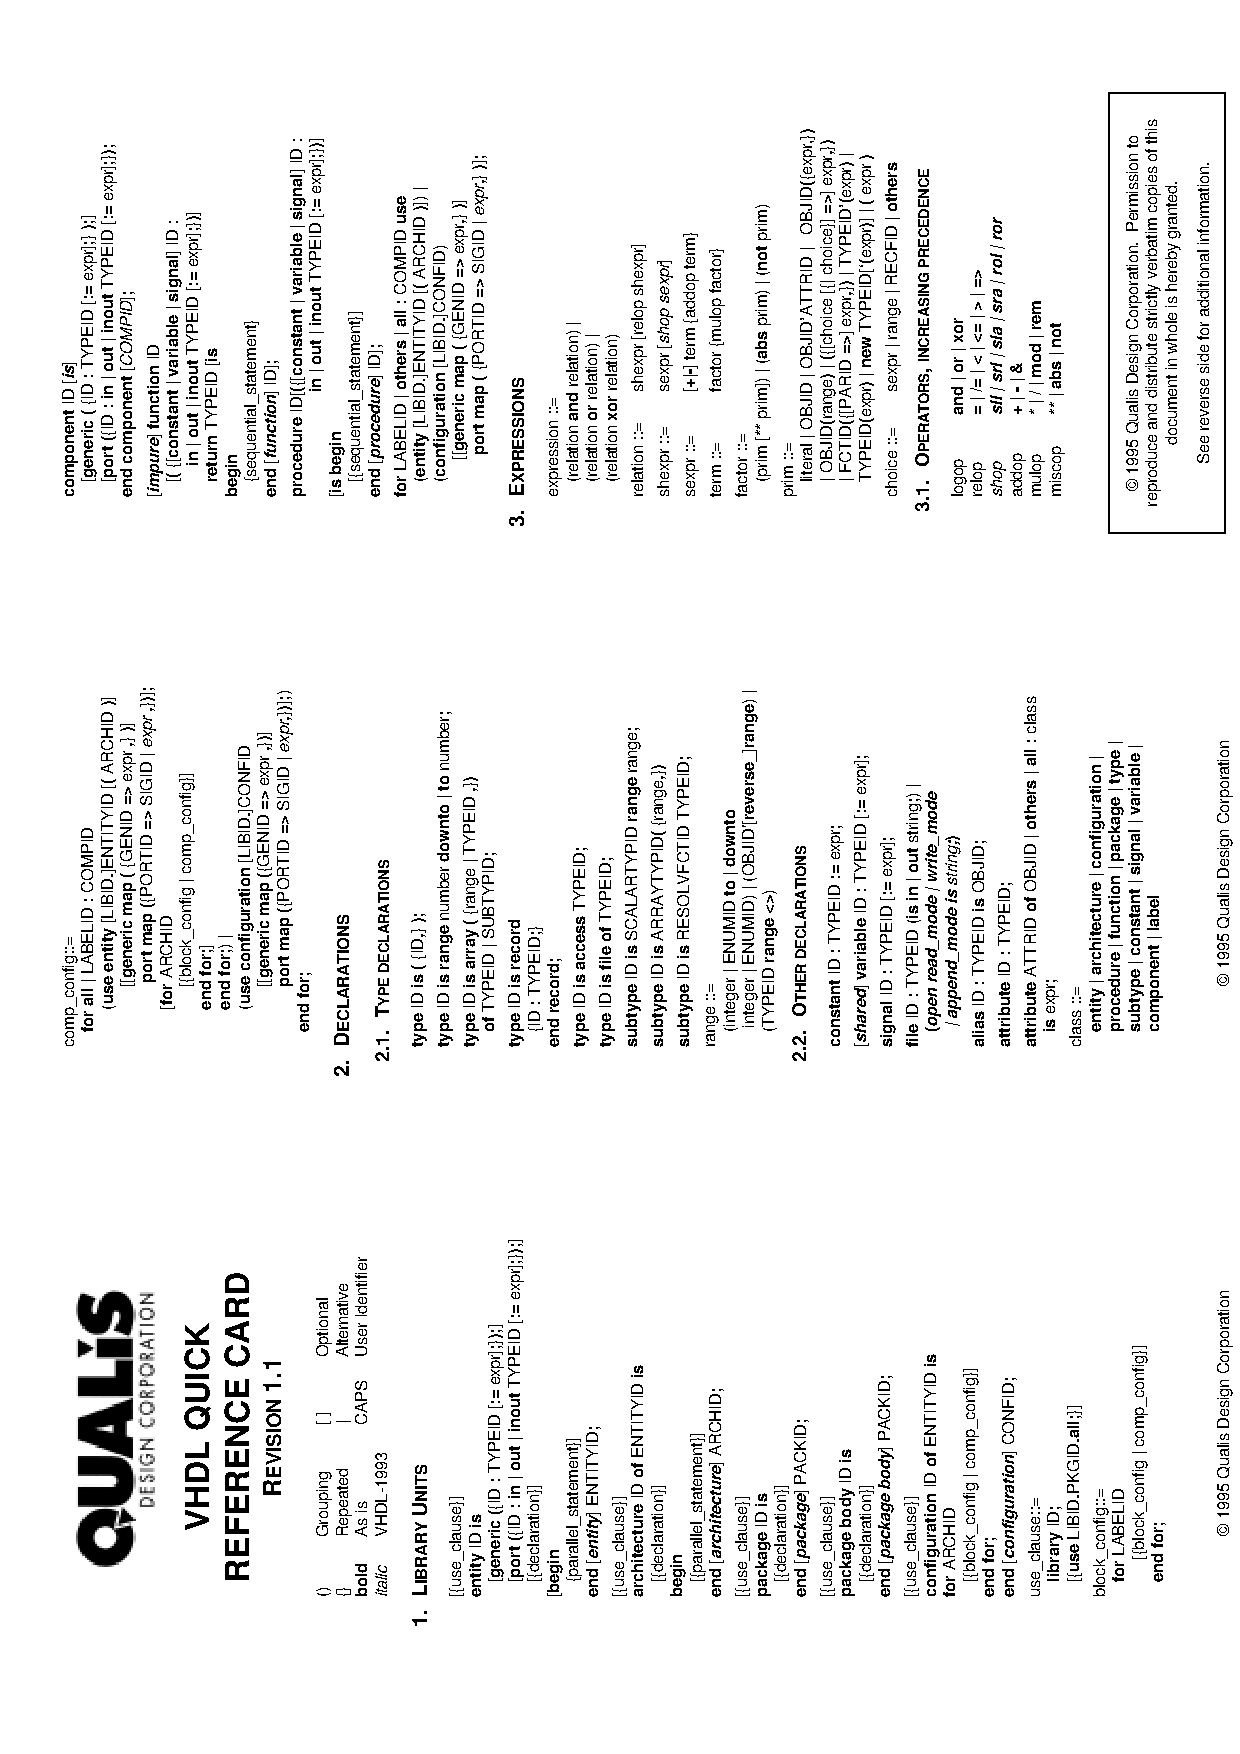
\includegraphics[width=145mm]{ref_cards/qr1.pdf}
\end{textblock*}
\null\newpage

\thispagestyle{empty}
\begin{textblock*}{148mm}(1mm,10mm)
%\textblockcolour{red}
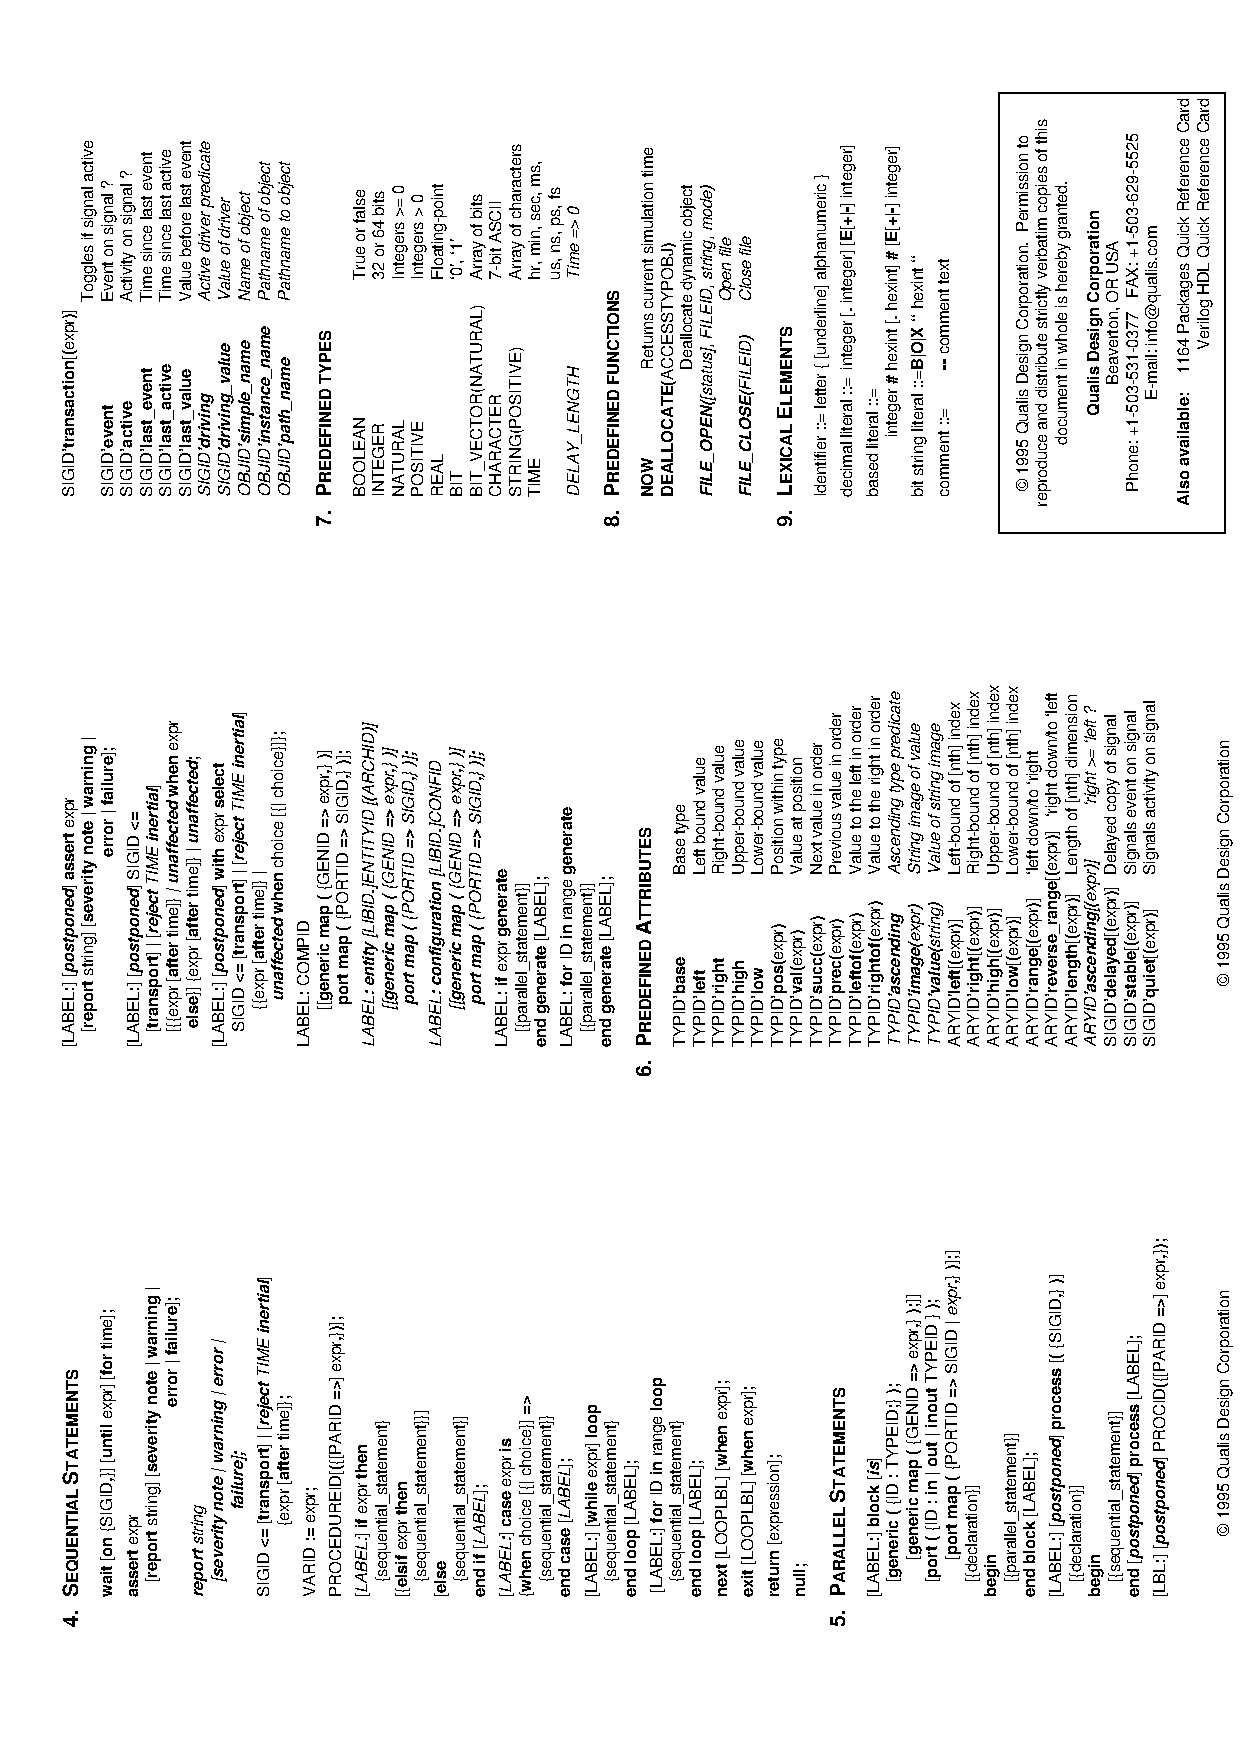
\includegraphics[width=145mm]{ref_cards/qr2.pdf}
\end{textblock*}
\null\newpage

\thispagestyle{empty}
\begin{textblock*}{148mm}(1mm,10mm)
%\textblockcolour{red}
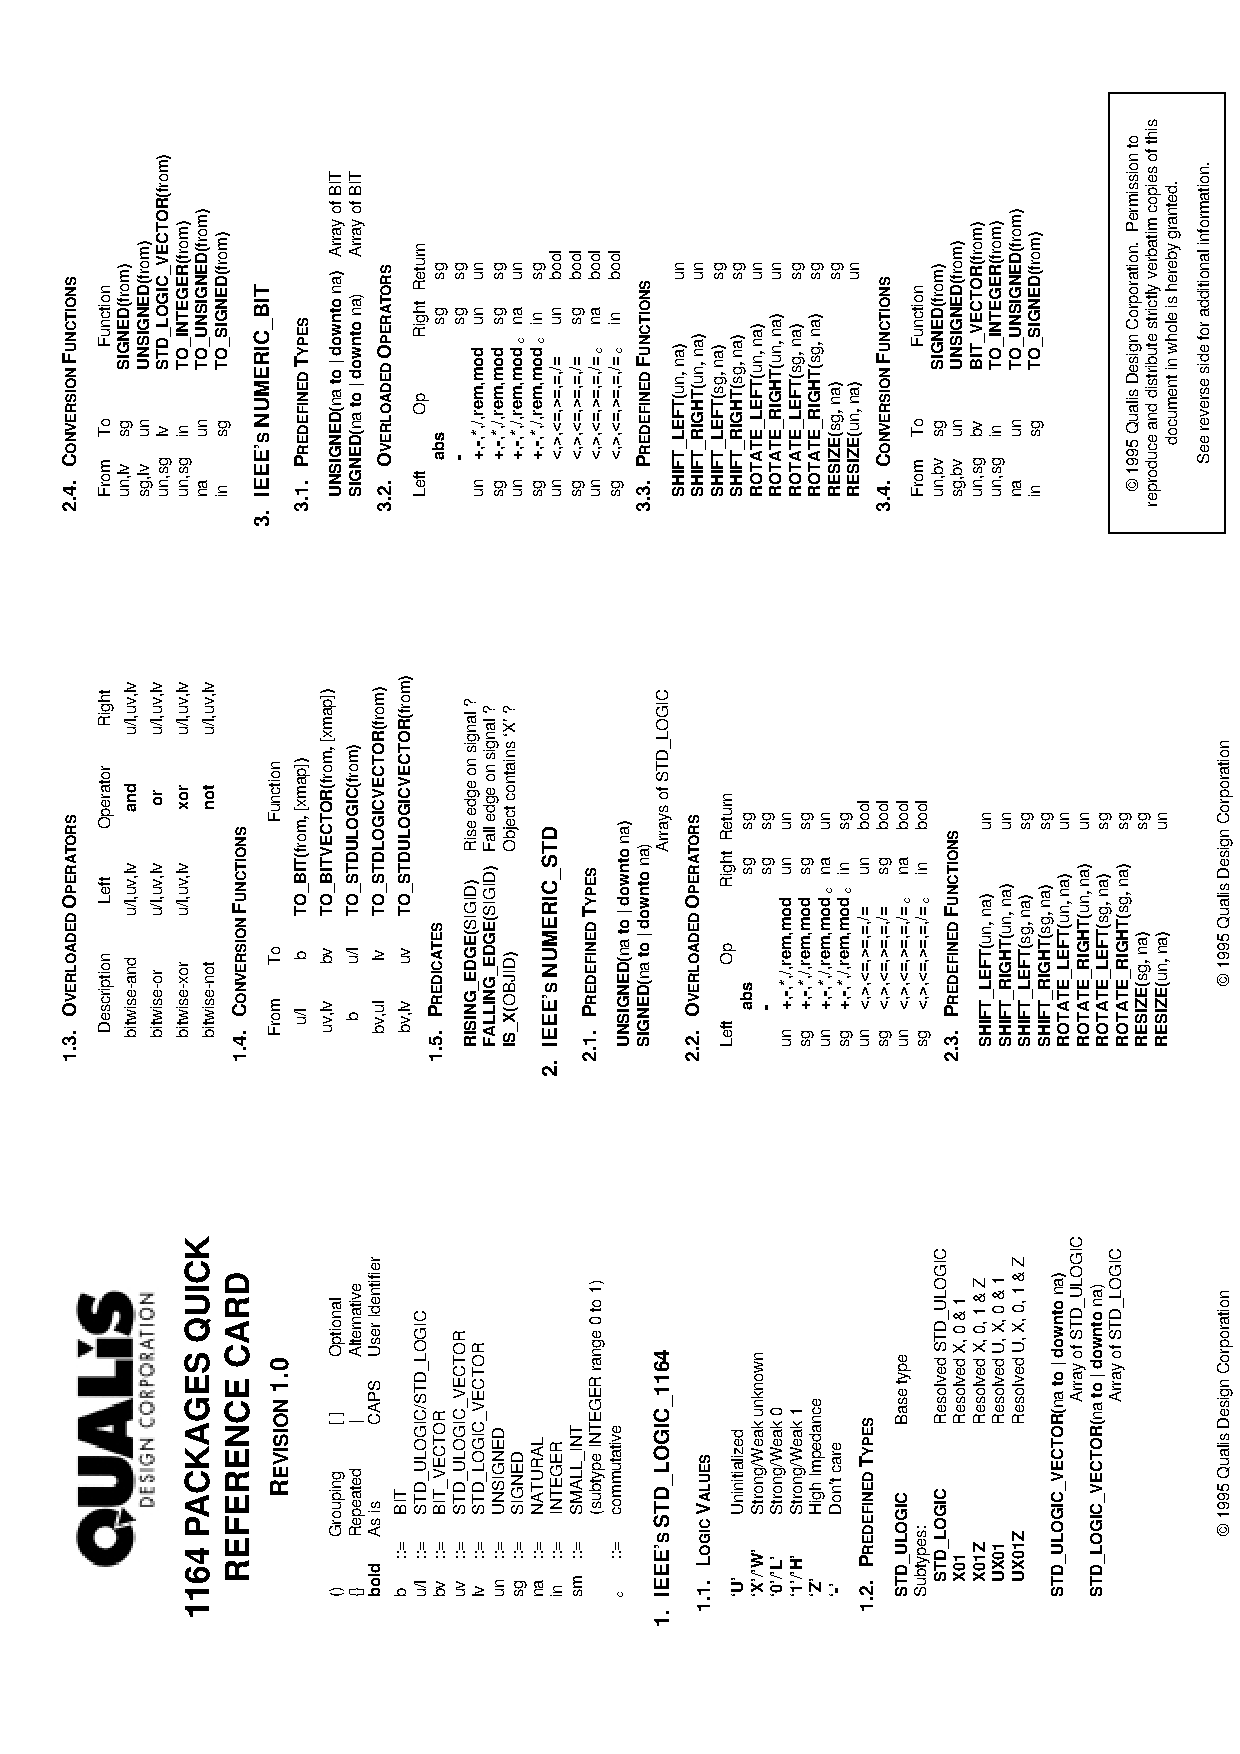
\includegraphics[width=145mm]{ref_cards/qr3.pdf}
\end{textblock*}
\null\newpage

\thispagestyle{empty}
\begin{textblock*}{148mm}(1mm,10mm)
%\textblockcolour{red}
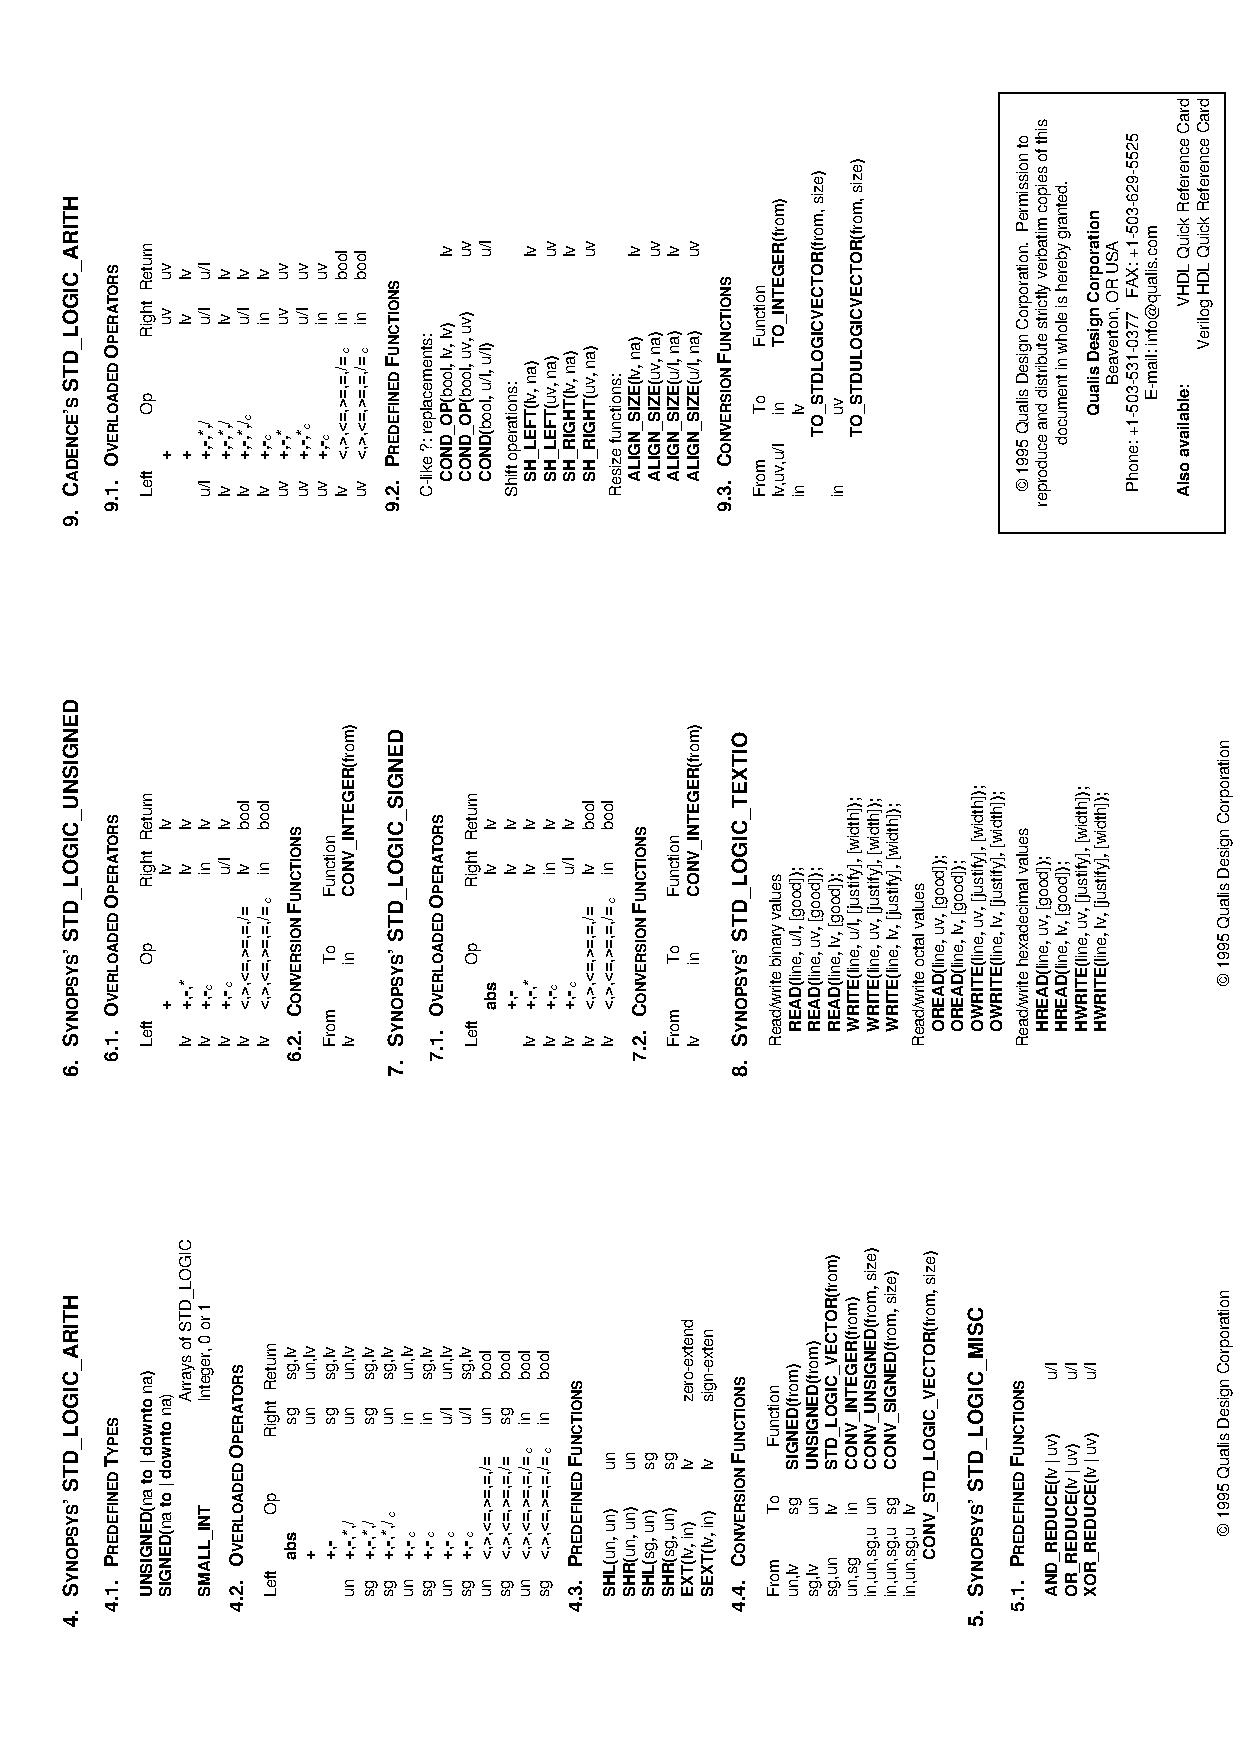
\includegraphics[width=145mm]{ref_cards/qr4.pdf}
\end{textblock*}
\null\newpage

